%%%%%%%%%%%%%%%%%%%%%%%%%%%%%%%%%%%%%%%%%%%%%%%%%%%%%%%%%%%%%%%%%%%%%%%%%%%%%%%%
%2345678901234567890123456789012345678901234567890123456789012345678901234567890
%        1         2         3         4         5         6         7         8

\documentclass[letterpaper, 10 pt, conference]{ieeeconf}  % Comment this line out
                                                          % if you need a4paper
%\documentclass[a4paper, 10pt, conference]{ieeeconf}      % Use this line for a4
                                                          % paper

\IEEEoverridecommandlockouts                              % This command is only
                                                          % needed if you want to
                                                          % use the \thanks command
\overrideIEEEmargins
% See the \addtolength command later in the file to balance the column lengths
% on the last page of the document



% The following packages can be found on http:\\www.ctan.org
\usepackage{graphics} % for pdf, bitmapped graphics files
\usepackage{graphicx,subcaption}
\usepackage[english]{babel}
%\usepackage[parfill]{parskip}
%usepackage{epsfig} % for postscript graphics files
\usepackage{mathptmx} % assumes new font selection scheme installed
\usepackage{times} % assumes new font selection scheme installed
\usepackage{amsmath} % assumes amsmath package installed
\usepackage{amssymb}  % assumes amsmath package installed
\usepackage{graphicx}
\graphicspath{ {./connectivityfractions/} }
\usepackage{diagbox}
\usepackage{slashbox}
\usepackage{float}
\usepackage{xfrac}
\usepackage[utf8]{inputenc}
\usepackage{fourier} 
\usepackage{array}
\usepackage{makecell}
\usepackage{caption}
\usepackage{url}
%\DeclareCaptionType{mycapequ}[][List of equations]
%\captionsetup[mycapequ]{labelformat=empty}

\usepackage[export]{adjustbox}

\renewcommand\theadalign{bc}
\renewcommand\theadfont{\bfseries}
\renewcommand\theadgape{\Gape[4pt]}
\renewcommand\cellgape{\Gape[4pt]}
\usepackage{cite}


\title{\LARGE \bf
Group Based Mobility Degradation Threshold Performance Comparison of MANET's On-demand Routing Protocols
}

%\author{ \parbox{3 in}{\centering Noah Omolaja David*
%         \thanks{*Use the $\backslash$thanks command to put information here}\\
%         Royal Holloway University of London, Information Security Department \\
%         University of Twente\\
%         7500 AE Enschede, The Netherlands\\
%         {\tt\small h.kwakernaak@autsubmit.com}}
%         \hspace*{ 0.5 in}
%         \parbox{3 in}{ \centering Pradeep Misra**
%         \thanks{**The footnote marks may be inserted manually}\\
%        Department of Electrical Engineering \\
%         Wright State University\\
%         Dayton, OH 45435, USA\\
%         {\tt\small pmisra@cs.wright.edu}}
%}

\author{Noah Omolaja David$^{1}$ and Stephen Wolthusen$^{2}$% <-this % stops a space
\thanks{*This work was not supported by any organization}% <-this % stops a space
\thanks{$^{1}$N. O. David is with the Information Security Department, Royal Holloway University of London,
        Egham Hill, TW20 0EX, United Kingdom 
        {\tt\small N. O. David at noah.okuonghae.2015@live.rhul.ac.uk}}%
\thanks{$^{2}$S. Woltusen is with the Information Security Department, Royal Holloway University of London, and 
        {\tt\small p.misra at ieee.org}}%
}


\begin{document}
\maketitle
\thispagestyle{empty}
\pagestyle{empty}
\begin{abstract}




%In Mobile ad hoc Networks (MANETs), some mobility metrics are directly related to the performance of routing protocols. Creating accurate predict models for mobility metrics is an important advance for designing better mobility-adaptive protocols. Through regression analysis, we propose predictive formulas for three mobility metrics: link duration, node degree, and network partitioning, considering a set of random, group, and grid-based mobility models. We propose specific derived parameters for group and grid-based models, and show that they are good predictors for the metric values. The results also show that link duration and node degree are more predictive for random and grid-based, and less predictive for group-based models.
Mobility patterns help us capture different mobility patterns used for evaluation of manet routing protocols. It is important that each different realistic and complex scenarios are captured in such evaluation, consideration should be given to different terrains and obstacles.

scenario outside of the often used RWP. various mobility patterns using mobility
During routing in manet, packets may be lost or corrupted as the network transition from


% introduction should talk about mobility models. Talk about importance of mobility models, most used RWP model and its limitation; failure to capture more complex scenarios like group mobility. Talk briefly about RPGM and introduce RPGM obstacle.
The performance of manet networks are significantly affected during transition 

In manet, node movement are dynamic and topological changes are unpredictable, often affecting the performance the performance of routing protocols \cite{Broch1998AProtocols}. Mobility among other factors have a significant deterministic attribute on the topology of manet. Mobility of manet nodes significantly impacts the performance of routing protocols \cite{Broch1998AProtocols}.

A lot of the research in manet have used (or on random waypoint model to evaluate the performancew of manet routing protocol. But to capture a more broad view of the true performance of this protocols multiple or other mobility models and scenarios must be captured. This paper, looks at group mobility using the MonnMotion RPGM and factors in scenario with obstacle using a new RPGM-obstacle to study the performance of Group mobility in reactive routing protocol.

% PAPER 2 : Mobility of manet nodes has a direct influence on the performance of routing protocols  and the value of impact also depends on the mobility model employed. Therefore, it is essential to have an understanding of the mobility model to be able to evaluate the effectiveness of the routing protocol (the effect of mobility on the performance of routing protocols).



Mobile ad hoc networks (Manets) are characterized by free, random and sporadic mobile nodes in the absence of any established infrastructure. Group mobility enjoy spatial dependency, hence movement of nodes are influenced by surrounding nodes. During route discovery, the relative influence of mobility, density and radio transmission range on entity nodes determines the connectivity of flat structure network scheme. Furthermore, transition from a connected to a partitioned network state will occur when updated routes to an intermediate node in the routing table becomes invalid for forwarding route discovery packets and the node is no longer reachable. This will trigger route maintenance, route error diffusion, and upper layer multi hop re-transmission thus increasing the routing overhead to an already resource constrained network. To minimize this degradation effect, we have compared the performance of three reactive MANET routing protocol AODV, DSR, AOMDV by using Group mobility and obstacle mobility. By comparing the performance of three reactive MANET routing protocols, Ad hoc on-demand Distance Vector (AODV), Dynamic Source Routing (DSR), Ad hoc On-demand Multi-path Distance Vector (AOMDV) by using Group mobility models of BonnMotion RPGM and an enhanced RPM obstacle mobility models. Even though these 3 protocols share similar on-demand behaviours, they are not designed routing algorithm does not prepare them for the eventuality of such graceful transitioning. We achieve these by investigating both qualitatively and quantitatively through simulation using NS-2, the impact of mobility, density and radio transmission range on the performance of Ad hoc on-demand Distance Vector (AODV), Dynamic Source Routing (DSR), Ad hoc On-demand Multi-path Distance Vector (AOMDV) using a novel network layer metric, connectivity fraction.  Our results does not only show us which on-demand routing protocol gracefully transition effectively under these network condition but we are able to predict each protocol's degradation threshold. This is important for optimizing the protocol's routing performance and conserving the network constrained resources




%Mobile ad hoc networks (Manets) may transition from a connected network state to a partitioned network state for certain reasons, some of which are predictable e.g. terrain and mobility factors or radio silence requirements, while others can be stochastic in nature or as a result of an attack e.g node compromise resulting in a black hole attack or jamming. During such transition in flat network topology, a degradation threshold is experienced where packets intended for forwarding to entity intermediate nodes are dropped, thus triggering route maintenance, route error diffusion, and upper layer multi hop re-transmission. However, these is costly as it increases the routing overhead to an already resource constrained network without providing any advance warning or indication of an impending network transition or topology change. This paper seeks to find out which Manet on-demand routing protocol would transitions effectively in such under provisioned condition. We study both qualitatively and quantitatively through simulation with NS-2, the performance of Ad hoc on-demand Distance Vector (AODV ), Dynamic Source Routing (DSR), Ad hoc On-demand Multi-path Distance Vector (AOMDV ). We investigate the fraction of connectivity from a source node to a destination node or across the network by a number of input parameters for mobility and partitioning: density, speed and radio transmission range using a novel network layer metric, connectivity fraction. Our results does not only show which of these 3 on-demand routing protocol transitions effectively, the rate at which degradation will occur, but also using logistic regression in WEKA, we are able to furthermore, predict the accuracy of our findings (predict if the degradation is reoccurring predictably or the predictive accuracy of our finding). These results are important for the selection of the most efficient on-demand protocol in an under provision topology and for future performance optimization of such protocol. 


%\IEEEpeerreviewmaketitle

\end{abstract}

% simple flooding, which could potentially lead to high channel contention, causing redundant retransmissions and thus excessive packet collisions in the network. This phenomenon has been shown to greatly increase the network communication overhead and end to end delay.


%In [13], Royer et al studied the optimum density of MANETs for stationary nodes. The proposed optimum density for keeping the stationary nodes connected in a network does not considered the effect of node mobility. 




%Such behavior has been known to mathematicians for sev-eral decades in the form of “zero-one” laws in Bernoulli Ran-dom Graphs. The basic idea is that for certain monotone graphproperties such as connectivity, as we vary the average densityof the graph, the probability that a randomly generated graphexhibits this property asymptotically transitions sharply fromzero to one at some critical threshold value



\section{INTRODUCTION}
Manets enjoy quick network setup and are among the most populous wireless ad hoc networks, often attracting with it a lot of research attention. It is synonymous with 1973 Defense Advanced Research Projects Agency (DARPA's) Mobile Packet Radio Networking\cite{Jubin1987TheProtocols}. One of it's major characteristic when compared to traditional wired networks, is it's sporadic mobility of nodes. Some Manet applications includes tactical operations, emergency search and rescue operations, as well as disaster recovery, collaborative and distributed mobile computing. The ease of these nodes to freely move about brings with it the challenge of effective and reliable routing, especially, in a resource constrained network like manet. This is attributed to its absent pre-existing communication infrastructure ad hoc network nature (see fig.\ref{fig:partition1}), where participating nodes cooperating in a friendly manner within minimal transmission range engage in multi-hop packet forwarding. The frequent change in topology caused by moving nodes results in the disruption of established routes, packet losses and substantial degradation of network services \cite{Su2001MobilityNetworks}. These communication complexities are managed by the routing protocols, which decides the best suitable route link to transmit data packet from the route initiated source mobile node to the targeted mobile node. Effective and reliable routing is usually a critical and challenging task, and the main function of the network layer.  This paper seeks to tackle the problem of network partitioning in multi hop on demand routing protocol, bringing about degradation in connectivity and the routing protocols overall performance, and eventually network partitioning. 

These papers have not addressed an important question about on-demand routing protocols and that is what at what point do nodes in on-demand routing protocol begin to transition from a connected network state to a partitioned state.% where nodes with random sporadic mobility transition into isolation thus initiating broken or lost paths as a result of poor/bad connectivity.

Although  we have focused on comparing the performances of three of the most popularly researched on-demand routing protocol AODV \cite{Mar
inaAdRouting}\cite{Perkins1999Ad-hocRouting}, DSR \cite{JohnsonDSR:Networks} and AOMDV \cite{MarinaAdRouting} by investigating a number of parameters for partitioning (density, mobility and radio transmission range) using a novel network metric connectivity fraction, we also analyze the simulation results to introduce a simple degradation threshold model. The degradation threshold model encourages localized route link association strategy in response to consistent transition from connected to partitioned network state. Conclusions from our analysis demonstrates that we are able to pre-determine (predict) an event of a change in topology for each protocol (see fig.\ref{fig:partition1}), based on if it is about to gracefully transition from a connected to partitioned network state and possible initiate a more robust or fault tolerant algorithm to maintain effective route link association or connectivity.


%To thoroughly and systematically study a new Mobile Ad hoc Network protocol, it is important to simulate this protocol and evaluate its protocol performance.% our results demonstrates that effective and reliable multi-hob routing are operational at this stage, subsequently to avoid partitioning, a more fault tolerant application (algorithm) must be activated to maintain effective routing and connectivity. %The scope of this paper is, however, not limited to  performance comparison of three on-demand  reactive routing protocols (DSR, AODV and AOMDV) by investigating a number of parameters for mobility and partition using the network matric, connectivity fraction. But also , how entity nodes in sparse and semi dense networks scenarios transition between connected and partitioned network states. 
The rest of the paper is organized as follows, Section II, performance study: related work in this area, with focus on AODV, DSR \& AOMDV, describes/introduces network model, the impact of mobility, density \& radio transmission range on the performance of on-demand routing protocol (algorithms) and partitioning. Section III, methodology:  describes the simulation parameters, performance metrics: connectivity fraction, Logical regression, accuracy graphs, degradation threshold model \& prediction table. Section IV, Result analysis. Section V, conclusion. Section VI, outlook to future work.

\begin{figure}[H]
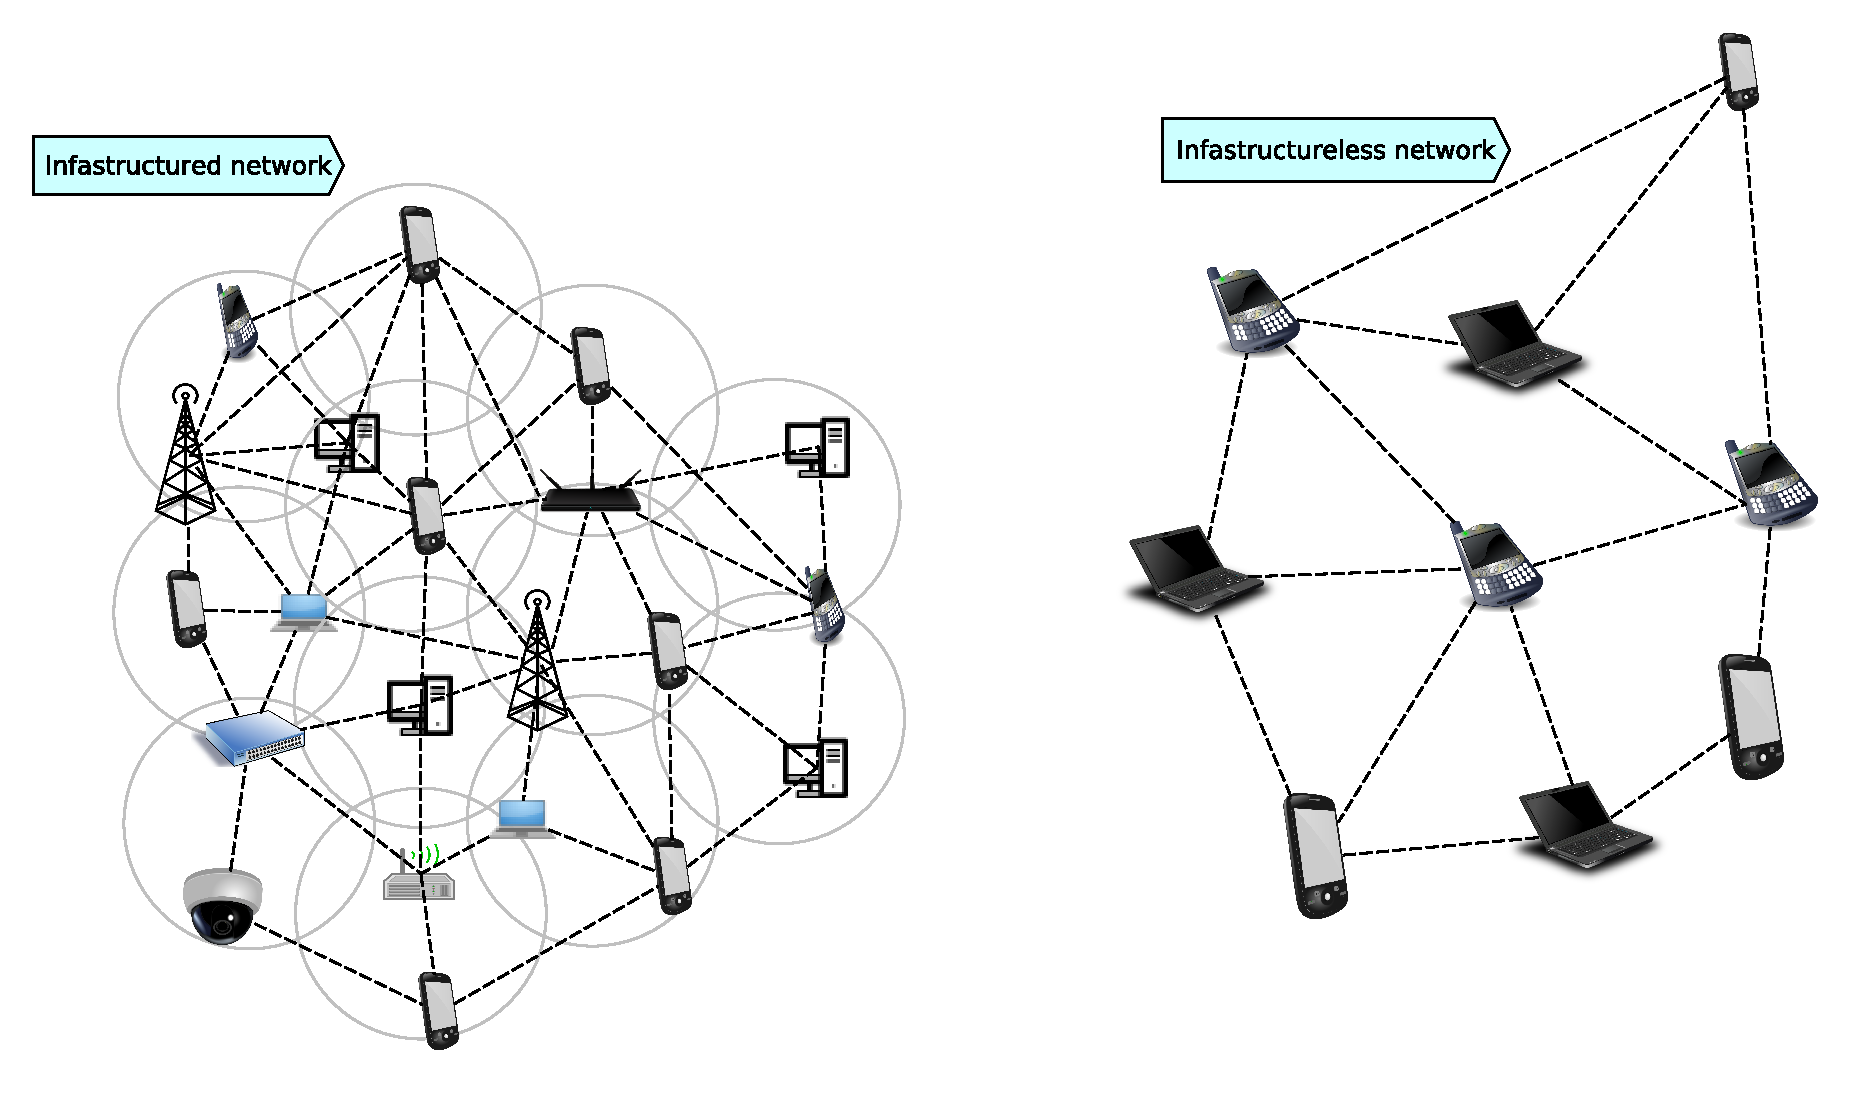
\includegraphics[width=0.45\textwidth]{infastructurelessNetwork1}
\caption{Wireless Networks}
\label{fig:infastructurelessNetwork1}
\end{figure}

% See figure \ref{fig:infastructurelessNetwork1} and on page \pageref{fig:infastructurelessNetwork1} %\newpage
%We perform a systematic study of wireless ad hoc networks with sparse and semi-dense density with average speeds which can potentially lead to frequent network partitions and focus primarily on their impact on data management algorithms.
\section{Performance Study}
A number of extensive simulation studies on various MANET
routing protocols have been performed by various researchers
[25][5][16][8][7]. However, there is a severe lacking in implementation
and operational experiences with existing MANET
routing protocols. Previous implementation experiences include
wireless Internet gateways (WINGS) [11], implementation
of ODMRP [2], AODV implementation by Royer et
al. [24] and ABR implementation by Toh et al. [27]. These
studies only highlighted performance issues specific to the
protocol being used. By far the most extensive implementation
study to date was conducted by Maltz et al. [17] in
describing their implementation of DSR.
Unlike previous work, our work reports on the experience
of building an operational ad-hoc network that is capable
of carrying useful data. We report several interesting observations
not reported elsewhere for the use of MANET
protocols within pico-cell environments. It is worthwhile
noting that this paper’s objective is to report on the operational
feasibility of existing routing protocols and efforts undertaken
to create a reliable ad-hoc network. In many ways
this is a step back towards fundamental issues and away from
the MANET routing protocol aspects usually examined in
simulation studies. Whereas simulation studies commonly
report on performance metrics such as throughput, latency
and packet loss this paper reports on the fundamental issue
of “do MANET routing protocols work”. The answer is yes
but, in the case of the two distance vector protocols we examined,
only if the inherent unreliable and transient nature
of wireless network links are taken into account.
\subsection{Related work}


\cite{Bai2004ModelingProtocols} \cite{Bai2003IMPORTANT:NeTworks}
Certain key parameters influence the performance of manet routing protocols and create a deterministic effect on reasons why manet may be partitioned. One of such parameters is mobility, which signifies how each single entity node moves, it location, velocity and acceleration change within an interval time. Mobility models are characterized by their spatial (a measure of how two nodes are dependent in their motion), temporal (a measure of how current velocity (magnitude and direction) are related to previous velocity), and geographic (a measure of how a node is confined to boundaries) dependencies. Therefore, choosing a realistic mobility scenario for network simulations plays an important role on the validity of the simulation as each routing protocol perform differently for different mobility model \cite{Broch1998AProtocols}, \cite{Perkins2001PerformanceNetworks}, \cite{DasComparativeNetworks}. An inherent problem with is the location management which produces a significant amount of overhead traffic. Therefore the routing to protocol to enjoy reliable and effective optimal routing performance, the routing algorithm mechanism (route discovery and maintenance) must be controlled \cite{Online2004ANetworks}. In order to isolate the effect of mobility, we fix the communicating traffic pattern to consist of randomly chosen source-destination pairs with long enough session times \cite{Bai2003TheNeTworks}. One of the goals IETF Mobile Ad Hoc Network group routing in manet  are to efficiently to topological changes and traffic demands while maintaining effective routing in a mobile networking context.
Radio transmission range plays a vital role on how nodes communicate and in turn influences the routing protocol's performance, therefore the consideration and implementation of a precise radio propagation model is important for achieving a more realistic performance evaluation 

\subsubsection{Multihop}

The utility of hello messages for determining link connectivity- Chakeres I Belding-Royer E


%Deterministic effects have a threshold below which the effect does not occur.%The mobility of the nodes affects the number of average connected paths, which in turn affect the performance of the routing algorithm


 




% Routing protocols like DSR [2], DSDV [3], AODV [4] and TORA [9] were mainly evaluated based on the following metrics: packet delivery ratio (ratio of the number of packets received to the number of packets sent) and routing overhead (number of routing control packets sent). [6] concluded that on-demand protocols such as DSR and AODV performed better than table driven ones such as DSDV at high mobility rates, while DSDV performed quite well at low mobility rates. [7] performed a comparison study of the two on-demand routing protocols: DSR and AODV, using the performance metrics of packet delivery ratio and end to  end delay. It observed that DSR outperforms AODV in less demanding situations, while AODV outperforms DSR at heavy traffic load and high mobility. However, the routing overhead of DSR was found to be lesser than that of AODV. In the above works, focus was given on performance evaluation, while parameters investigated in the mobility model were change of maximum velocity and pause time. In our work, however, we design our test suites very carefully to pick scenarios that span a much larger set of mobility characteristics. Not only do we use Random Waypoint but also other mobility models such as RPGM [5], Freeway and Manhattan in our evaluation of the performance of routing protocols.

 



Some Manet routing protocol performance evaluation has been proposed in research literature

\textbf{Mobility and density: the impact of mobility has been studied over time} 

mobility have significant impact on partitioning and characterization of of their behavior helps improve the performance of distributed algorithms. The studied networks with low node density capable of leading to frequent network partitions and focus primarily on their impact on data management algorithms. \cite{Hahner2007QuantifyingNetworks}


\textbf{stop}

we only focus on developing a detailed approach to study the effect of mobility on the performance of reactive MANET routing pro tocols like dynamic source routing (DSR) [3] and ad hoc on-demand distance vector (AODV) \cite{Bai2004ModelingProtocolsb}





%Popular simulators use mobility models to generate movement patterns for wireless-hosts. The mobility models,therefore, must imitate practical scenarios close enough for the simulators to provide realistic performance measurements.


% Research in mobility modeling is performed in two directions. The first direction (primary research direction until 2000) is to design new models in order to mimic the real  world scenarios better. The second direction (predominant afterwards) is to analyze these models. This includes finding the statistical properties of the
 mobility models, designing
different mobility metrics and studying the influences of mobility models on routing protocols’ performance. An earlier survey on mobility models can be found in



The failure of set of links or nodes in the underlying network can cause the network to break away into two or more components or
clusters,  As a result of this, nodes within a cluster can communicate each other, but there is no communication across the nodes in different cluster. This phenomenon is called network partitioning, . Protocols in Manets are categorized into 3 major groups, namely reactive, proactive and high- breed





\subsubsection{Routing in Manet: impact of density, speed, mobility and radio transmission range on performance of Manet, prediction and degradation threshold. What we propose:other's network metrics like pdf but we use connectivity fraction
 used pdf}
\textbf{We argue that figuring out when two nodes
will meet with a probability distribution could improve the
delivery ratio, as well as reduce the delivery latency}



 When a source node S needs to communicate with a destination node D, it sends out broadcast control discovery message to nearby neighbor nodes covered in its transmission range




\cite{BrochAProtocols}This paper presented a mre realistic, quantittative analysis comparing the performance of a variety of multihop wireless ad hoc routing protocols( DSDV, TORA, DSR, AODV.

Transmission range and network size have significant influences on the performance on manet routing protocols.\cite{Belding-Royer2002TransmissionCommunication} explored/investigated the effects of transmission on AODV's multicast performance using different transmission ranges of 200 to 500 meters and network configurations. Noting
 that network partitions occurred more when transmission ranges where lower than 200 m, making it difficult for accurate comparison as result of sparse network connectivity. Their results concluded that A larger transmission radius results in
better packet delivery ratio, fewer link breaks in the multicast tree, and less control overhead and thus overwhelm system resources like battery power.




 A communication session is achieved either
through single-hop transmission if the recipient is
within the transmission range of the source node,
or by relaying through intermediate nodes otherwise.
For this reason, MANETs are also called
multi-hop packet radio networks. However, the
transmission range of each low-power node is limited
to each other’s proximity, and out-of-ran
ge
nodes are routed through intermediate nodes.




%studied the effects of transmission range on AODV’s multicast performance by examining the results achieved at varying transmission ranges and network configurations. In order to explore the effects of transmission range, seven different ranges, from 200 m to 500 m, are studied. Shorter than 200 m, network connectivity is too sparse for an accurate comparison, as network partitions occur. The results of the 450 m and 500 m simulations are similar enough to be able to extrapolate the effects of further increasing the transmission range. Each transmission radius/speed combination was run for ten different initial network configurations. she used  seven different transmission ranges modeled. First packet delivery ratio; an increase in range yields an increase in the packet delivery ratio, or the number of data packets received by multicast group members. Having examined only these results, it appears that in-creasing the transmission radius has a uniformly positive effect on the network. A larger transmission radius res
ults in better packet delivery ratio, fewer link breaks in the multicast tree, and less control overhead. The transmission range and network size are key determinants of AODV’s multicast performance. We conclude that the transmission range should be adjusted to meet the targeted throughput while minimizing battery power consumption.We hope that this exploratory work on the relationship between transmission ranges and multicast routing performance will lead the way towards improving the reliability of best-effort multicast packet delivery. We conclude that the transmission range should be adjusted to meet the targeted throughput while minimizing battery power consumption. Our work shows that there are opportunities for power savings when nodes can get the same (or even better) performance by reducing the power drain caused by unnecessarily high transmission ranges.






%Several factors will affect the overall 
performance of any protocol operating in an ad hoc network. For example, node mobility may cause link failures, which will negatively impact routing and quality-of-service support. Network size, control overhead, and traffic intensity will have a considerable impact on network scalability. These factors along with inherent characteristics of ad hoc networks may result in unpredictable variations in the overall network performance.

Moreover, mobility is also expected to affectDeleted 

the service quality significantly. For example, the frequent
topology changes caused by node movement in high mobility
scenarios may result in the disruption of established routes,
leading to packet losses and substantial degradation of service
quality. Thus, in order to design paradigms of service quality in
MANETs, it is essential to understand the impact of mobility
on performance.
 A communication session is achieved eith
er
through single-hop transmission if the recipient is
within the transmission range of the source node,
or by relaying through intermediate nodes otherwise.
For this reason, MANETs are also called
multi-hop packet radio networks. However, the
transmission range of each low-power node is limited
to each other’s proximity, and out-of-range
nodes are routed through intermediate nodes.



 It uses statistical
analysis (of simulation data) to obtain detailed statistics of link
and path duration including their probability density functionsDeleted 
Feb 20, 2019 8:29 AM • You
(pdfs). Through simple analytical models, using the case study
of DSR, it shows a strong correlation between the reciprocal
of average path duration and  A communication session is achieved either
through single-hop transmission if the recipient is
within the transmission range of the source node,
or by relaying through intermediate nodes otherwise.
For this reason, MANETs are also called
multi-hop packet radio networks. However, the
transmission range of each low-power node is limited
to each other’s proximity, and out-of-range
nodes are routed through intermediate nodes.the throughput and overhead of
reactive protocols. Further, the approach uses a case study of
DSR to demonstrate how the path duration pdf can be used to
analytically determine the nonpropagating cache hit ratio in the
freeway mobility model.



 In this paper, we ex-
amine the detailed statistics of link and path duration including
pdfs across the “test-suite” of mobility models proposed in [21].
We then attempt to categorize the relationship between the av-
erage path duration and protocol performance as either strongly
(or weakly) linearly (or nonlinearly) related. We also relate the
path duration pdfs to the im A communication session is achieved either
through single-hop transmission if the recipient is
within the transmission range of the source node,
or by relaying through intermediate nodes otherwise.
For this reason, MANETs are also called
multi-hop packet radio networks. However, the
transmission range of each low-power node is limited
to each other’s proximity, and out-of-range
nodes are routed through intermediate nodes.pact of mobility on the “building
blocks” of reactive protocols. \cite{Bai2004ModelingProtocolsb}

\textbf{stop}
% A number of works [10,7,4,11,15,8] have stressed two of the main differences: the prevalent mode of communication in wireless networks is broadcast, and the network topology can change spontaneously. The latter point implies that there is a strict separation A communication session is achieved either
through single-hop transmission if the recipient is
within the transmission range of the source node,
or by relaying through intermediate nodes otherwise.
For this reason, MANETs are also called
multi-hop packet radio networks. However, the
transmission range of each low-power node is limited
to each other’s proximity, and out-of-range
nodes are routed through intermediate nodes. between process actions and the mobility modelling, since changes in connectivity are influenced by environment conditions (such as node movement), but not by the actions ofa protocol process.


\textbf{Mobility review}
% Related work -------- https://onlinelibrary.wiley.com/doi/full/10.1002/wcm.72


%The mobility model is designed to describe the movement pattern of mobile users, and how their location, velocity and acceleration change over time.


This paper proposes a novel approach to understand the
effect of mobility on protocol performance. It uses statistical
analysis (of simulation data) to obtain detailed statistics of link
and path duration including their probability density functions
(pdfs). Through simple analytical models, using the case study
of DSR, it shows a strong correlation between the reciprocal
of average path duration and the throughput and overhead of
reactive protocols. Further, the approach uses a case study of
DSR to demonstrate how the path duration pdf can be used to
analytically determine the nonpropagating cache hit ratio in the
freeway mobility model.


Recently, there has been a greater focus on a systematic
study of the effect of mobility on the performance of routing
protocols. Reference [21] proposed the IMPORTANT framework
to systematically analyze the effect of mobility on routing
protocols. In this framework, the authors proposed to evaluate
the MANET routing protocols using a “test-suite” of
mobility models that span several mobility characteristics like
spatial dependence, geographic restrictions, etc. These models
included the random waypoint (RW), reference point group
mobility (RPGM), freeway (FW), and Manhattan (MH). They
found that mobility significantly impacts the performance of
the protocols, which is in agreement with several other studies.
Moreover, they also proposed a reason for why mobility impacts
performance: Mobility impacts the connectivity graph (average
link duration in particular), which in turn impacts the protocol
performance.
To explain how mobility impacts the performance, [22] introduced
the BRICS methodology. It proposed that a protocol
could be considered to be made up of parameterized “building
blocks” or basic mechanisms. The effect of mobility on the entire
protocol can be explained in terms of its effect on these
“building blocks.” Some of the “building blocks” proposed by
BRICS for reactive protocols were flooding, caching, error detection,
error notification, and error recovery. Both DSR and
AODV use these “building blocks” in their operation. However,
they still behave differently for a given mobility model. BRICS
suggested that a possible reason for this difference might be the
different parameter settings for the “building blocks” in AODV
and DSR. This leads to different impacts of mobility on these
mechanisms. A brief overview of the work done in [21] and [22]
\cite{Bai2004ModelingProtocols}
\textbf{Stop}

However, systematic performance evaluations and comparative analysis of these protocols in a common realistic environment has not yet been performed. In this study, we simulate a set of representative wireless ad hoc multicast protocols and evaluate them in various network scenarios. The relative strengths, weaknesses, and applicability of each multicast protocol to diverse situations are
studied and discussed. 


 this paper is the first to conduct
a performance comparison study of ad hoc wireless multicast
protocols in a realistic common simulat A communication session is achieved either
through single-hop transmission if the recipient is
within the transmission range of the source node,
or by relaying through intermediate nodes otherwise.
For this reason, MANETs are also called
multi-hop packet radio networks. However, the
transmission range of each low-power node is limited
to each other’s proximity, and out-of-range
nodes are routed through intermediate nodes.ion environment. By using
a detailed simulator, we provide quantitative performance
analysis of five protocols with different characteristics: AMRoute
[3], ODMRP [17], [18], [19], AMRIS [29], CAMP [lo],
[ 111, [21], [22], and flooding. In addition to multicast routing
protocols, we also implemented a detailed and realistic model of
physical and medium access control layer protocols.
The five multicast routing protocols were simulated in diverse
network scenarios. We studied the impact of mobility on performance
by varying the speed of network hosts. We varied the
number of data packet senders to emulate a variety of different
multicast applications. One source to many receivers can correspond
to battlefield data dissemination. Many sources to many
receivers can correspond to search and rescue team communication.
Different multicast group member sizes were simulated
to investigate the impact on performance. Various traffic loads
were also applied to study how traffic patterns influence multicast
protocol performance. We apply metrics that show the
“efficiency” in addition to the “effectiveness” of the protocols.
Understanding the protocol’s efficiency gives us the ability to
study and discuss relative strengths, weaknesses, and applicability
to various situations for each multicast routing protocol.



Advances in packet radio networks, each adapted for their special requirements imposed on it. Their design capture not only operational requirements but also environmental constraints \cite{Ephremides1987ASignaling} \cite{Gerla1995MulticlusterNetwork} This radio network is not supported by a wired infrastructure as conventional cellular systems are. Thus, it can be instantly deployed in areas with no infrastructure at all. By using a distributed clustering algorithm, nodes are organized into clusters. The cluster heads act as local coordinators to resolve channel scheduling, perform power measurement/control, maintain time division frame synchronization, and enhance the spatial reuse of time slots and codes.





The features that distinguish this network from other
packet radio (PR) networks stem from the special operational
requirements and environmental constraints that it
must satisfy. Briefly, these consist of the following:
1) A relatively small number of nodes (2 to IOO), which
are mobile and whose connectivities may change dynamically
as a result of variable propagation conditions and interference,
must remain connected.
2) These nodes must be able to communicate to points
both within and outside the network under a variety of op
erating modes and scenarios.
3) The network must be secure, must resist a variety of
jamming threats, and must be able to degrade gracefully
under conditions of stress.
4) Both voice and data communications must be sup
ported, including point-to-point and broadcast transmissions,
while accommodating various precedence levels. 



\textbf{Impact of mobility on routing protocol performance:}


\textbf{Factors that influence Connectivity}


Randomization of Nodes: mobility Definition and how it affects connectivity In general, a multi-hop network tries to find a route between a source and a destination to forward the information. 











Metrics
We have used the following metrics in comparing protocol
performance. Some of these metrics were suggested by the IETF
MANET working group for routing/multicasting protocol evaluation
[SI.
Packet delivery ratio: The ratio of the number of data packets
actually delivered to the destinations versus the number of
data packets supposed to be received. This number presents the
effectiveness of a protocol.
Number of data packets transmitted per data packet delivered:
‘Data packets transmitted’ is the count of every individual
transmission of data by each node over the entire network.
This count includes transmissions of packets that are eventually
dropped and retransmitted by intermediate nodes. Note that in
unicast protocols, this measure is always equal or greater than
one. In multicast, since a single transmission can deliver data to
multiple destinations, the measure may be less than one.
Number of control bytes transmitted per data bytes delivered:
Instead of using a measure of pure control overhead,
we chose to use the ratio of control bytes transmitted to data
bytes delivered to investigate how efficiently control packets are
utilized in delivering data. 

\cite{Lee2000AProtocols}
\textbf{Stop}

% they AODV, DSR and AOMDV all initiate routing activities on an “on demand” basis. This reactive nature of these protocols is a significant departure from more traditional proactive protocols, that find routes between all source-destination pairs regardless of the use or need of such routes. The key motivation behind the design of on-demand protocols is the reduction of the routing load. High routing load usually has a significant performance impact in low bandwidth wireless links 
\cite{DasPerformanceNetworks}


% LITERATURE REVIEW: We compare the performance of two prominent on-demand routing protocols for mobile ad hoc networks — Dynamic Source Routing (DSR) and Ad Hoc On-Demand Distance Vector Routing (AODV). A detailed simulation model with MAC and physical layer models is used to study inter-layer interactions and their performance implications. We demonstrate that even though DSR and AODV share a similar on-demand behavior, the differences in the protocol mechanics can lead to significant performance differentials. The performance differentials are analyzed using varying network load, mobility and network size



%During routing in wireless ad hoc networks, connectivity is determined by the reception of broadcast control messages and a 

%Scenario like tactical military networks \cite{AschenbruckANetworks}

%Network connectivity may be determined through the reception of broadcast control messages. Any broadcast control message also serves as a hello message, indicating the presence of a neighbor. When a node receives a hello message from its neighbor, it creates or refreshes the routing table entry to the neighbor. To maintain connectivity, if a node has not sent any broadcast control message within a specified interval, a hello message is locally broadcast. This results in at least one hello message transmission during every time period. Failure to receive any hello message from a neighbor for several time intervals indicates that neighbor is no longer within transmission range, and connectivity has been lost. Two variables control the determination of connectivity using hello messages: HELLO INTERVAL and ALLOWED HELLO LOSS. HELLO INTERVAL specifies the maximum time interval between the transmission of hello messages. ALLOWED HELLO LOSS specifies the maximum number of periods of HELLO INTERVAL to wait without receiving a hello message before detecting a loss of connectivity to a neighbor. The recommended value for HELLO INTERVAL is one second and for ALLOWED HELLO LOSS is two [11]. In other words, if a hello message is not received from a neighbor within two seconds of the last message, a loss of connectivity to that neighbor is determined.


%Network connectivity may be determined through the reception broad cast control message. A network is said to be partitioned when it has been split into two or more subsystems that lack any connections between them.





%The modeling of movement is an important role in analysis of algorithms and protocols of wireless networks\cite{Camp2002AResearAch} and \cite{Navidi2003Stationary} (state) that the performance results of an ad hoc network protocol + significantly change when the mobility model in the simulation is changed. The results presented prove the importance of choosing an appropriate mobility model (or models) for a given performance evaluation. 

Also \cite{Bai2004ModelingProtocols}


% or For example a SEAL team in hostile enemy environment

% In the last decade, MANETs have been the focus of interest is several mobile deployments in both civilian and military environments.  Such deployments include a network of smart devices carried by members of armed forces in a battlefield, a network of wireless sensors deployed in an oil field (intelligent oil fields)



%\newline
%  comparing the relative performance of three key ad-hoc routing protocols: Destination-sequenced Distance Vector (DSDV), Ad-hoc On-demand Distance Vector (AODV) and Optimized Link State Routing (OLSR).  The protocols were tested based on two scenarios, namely, tactical networks for ships and sensor-based network nodes.  The objective is to validate the scalability and effectiveness of the protocols.  Four performance metrics were measured by varying the maximum speed of mobile hosts, network size and traffic load, to assess the routing capability and protocol efficiency.  The simulation results indicate that AODV performs better than OSLR and DSDV in the first scenario.  Although OLSR also performed relatively well, the associated high routing overhead is the dominant reason for not choosing it.


%used mobility model in the simulation of ad hoc networks


Cut from here(DETERMINATION OF NETWORK TOPOLOGY
An ad hoc routing protocol must determine and
monitor the dynamics of network topology over
time. Since multihop communications are needed
in ad hoc networks, the routing protocol must
ensure that links in the route have strong connectivity.
There must exist at least one path from
any node to any other node in a nonpartitioned
network. A node in the ad hoc network must be
aware of its surrounding environment and the
neighboring nodes with which it can directly
communicate. It must take into account the relative
difficulties of forming links with those nodes
and the benefits such connections will bring to
the network on the whole (e.g., bandwidth usage,
transmission delay, throughput, power consumption).
Basically, there are two approaches in providing
ad hoc network connectivity:
Hierarchical network architectures 
In the flat-routed network architecture, all the
nodes are equal and packet routing is done
based on peer-to-peer connections. However, in
hierarchical networks, at least one node in each
lower layer is designated to serve)


A review of current routing protocols for adhoc mobile wireless networks. IEEE Personal Communications, pages 46-55, April 1999--. Moreover, the overhead can have a significant impact on the overall
performance of the adhoc network. The movement pattern of MANET nodes is characterized by mobility models and each routing protocols exhibits specific
characteristics for these models --T. Camp et al. A survey of mobility models for adhoc network research. Wireless Communication and Mobile Computing (WCMC): Special issue on Mobile Ad-hoc Networking: Research, Trends and Applications, 2(5):483-502, 2002. (Pubitemid 135713186--. In order to find the most adaptive and efficient routing protocol for dynamic MANET topologies, the behavior of routing protocols needs to be
analyzed at varying node speeds, transmission range, network size, as well as node density --G. Lin, G. Noubir, and R. Rajaraman. Mobility models for adhoc network simulation. International Journal of Computer Science and Network Security, 7(6):160-164, 2007--. The node movement patterns differ for different scenarios; military adhoc networks.

Therefore, in this paper, we aim to analyze the performance of MANET routing agent AODV under the random waypoint  mobility model with the connectivity fraction network parameter . The paper is organized as follows. In Section II, we provide a brief overview of MANET routing protocols. Section III describes the different mobility models for MANETs. Section IV gives the details of our performance simulations for protocol evaluation along with their results and critical analysis. Our paper finally concludes in Section V with an outlook to future work.










%Every node in the network  is  capable  of  functioning  as a  mobile  router (maintain routes & forward packets), which makes possible the  multi-hop forwarding  of packets from a source node to  a destination node without reliance  on  a fixed  infrastructure.

How mobility impact reactive protocols \cite{SadagopanPATHS:Protocolsb} ( focus on developing a detailed approach to study the effect of mobility per
se on the performance of reactive MANET routing protocols like DSR [2] and AODV \cite{DasAdRoutingb} examines the statistic of path duration including PDFs varying with parameters such as the mobility model, relative speed, number of hops and radio range 

% The technology of Mobile Ad hoc Networking is somewhat synonymous with Mobile Packet Radio Networking (a term coined via during early military research in the 70's and 80's), Mobile Mesh Networking (a term that appeared in an article in The Economist regarding the structure of future military networks) and Mobile, Multi hop, Wireless Networking (perhaps the most accurate term, although a bit cumbersome).

% In 1973, the Defense Advanced Research Projects Agency (DARPA) initiated research on the feasibility of using packet switched, store-and-forward radio communications to provide reliable computer communications [I]. This development was motivated by the need to provide computer network access to mobile hosts and terminals, and to provide computer communications in a mobile environment. Packet radio networking offers a highly efficient way of using a multiple-access channel, particularly with bursty traffic [2]. The DARPA Packet Radio Network (PRNET) has evolved through the years to be a robust, reliable, operational experimental network [3]. The development process has been of an incremental, evolutionary nature [4]; as algorithms were designed and implemented, new versions of the PRNET with increased capabilities were demonstrated. he PRNET has been in daily operation for experimental purposes for nearly ten years

some
%Interest in such dynamic wireless networks is not new. It dates back to the seventies, when the US. Defense Research 

% My research looks at connectivity and partitioning, which focuses on the problem of routing in manet, just before packets are sent out.
ms of th

When evaluating the performance of protocols in adhoc networks (attempts must be made to ) realistic conditions should be considered in selecting radio transition range, buffer space for storage of messages, representative data traffic models and movement of the mobile users. Two major types of mobility models used in simulation of adhoc networks are the entity \cite{Camp2002AResearch} and group mobility models \cite{Hong1999ANetworks}. In this paper we focus on the random waypoint mobility model \cite{Navidi2004StationaryModel} which is an entity mobility models that is characterized by mobile nodes movements that are independent of each other and non-uniform.











\begin{figure}[H]
\includegraphics[width=0.45\textwidth]{partition1}
\caption{Network Partition}
\label{fig:partition1}
\end{figure}

%See figure \ref{fig:partition1} and on page \pageref{fig:partition1}





\subsection{Partitioning}


Decentralized and infastructureless wireless adhoc networks are basic features of manet's dynamic and ever changing topology. Mobile nodes route their packets through collaboration of intermediate nodes with the help of routing protocol. Routing protocols are broadly classified into: Reactive protocol, proactive protocol and hybrid routing protocols. Reactive routing protocols only send out rout

Mobile nodes route their packets through collaboration of intermediate nodes with the help of routing protocol. When a source node A needs to communicate with a destination node Z and does not have the route to the destination it initiates the route discovery process by locally broadcasting control messages to its nearby neighbor nodes C, B, D, X, B, E  within its transmission range  see fig.\ref{fig:partition1}. However, when one of these nodes (e.g C) moves away from the transmission range of the source node A, the route link becomes broken. This triggers a fresh route discovery process, which degrades the network connectivity and can eventually leads to a partitioned network if reestablishment of the route link fails. 

\subsection{Routing in manet}
Routing protocols are broadly classified into: Reactive protocol, proactive protocol and hybrid routing protocols. In reactive routing protocol, every node updates it's routing table on a need basis or in an event of a topology change by sending out route discovery request towards the destination node, hence it's called the on demand routing protocols. They are known to have relatively low routing overhead in comparison to proactive routing protocols thus have better scalability. However, long delays are experienced before packets are forwarded as result of time taken to query route information and update routing table. Examples of such protocols include AODV, DSR and AOMDV. In proactive routing protocol, every node updates it's routing table by periodically sending out route discovery requests to its surrounding neighbour nodes or even without being triggered by an event of topology change. Routes to destination node from source nodes are instantaneous than reactive routing protocols, as their routing tables are always update with current routes hence also known as table driven protocol. Proactive routing protocol can be overwhelmed by large overhead traffic during route maintenance in large networks as a result of their regular route updates. However, because they keep an upto date routing information table, routes are always available on request Examples of such protocols include Destination-sequenced distance vector (DSDV)\cite{Perkins1994HighlyComputers}, Fisheye state routing (FSR)\cite{GuangyuPeiFisheyeNetworks} and  Wireless routing protocol (WRP)\cite{Murthy1995ANetworks}. Hybrid routing protocol are protocols that harness the best qualities of both the reactive and proactive routing protocols. Examples of hybrid protocols include Zone Routing Protocol (ZRP) \cite{Haas2002TheNetworks} and AOMDV.
 
 


\subsubsection{Ad-hoc On-Demand Distance Vector}

AODV\cite{DasAdRouting} \cite{Perkins1999Ad-hocRouting} is an on demand routing protocol from variants of DSDV\cite{Perkins1994HighlyComputers} and DSR\cite{JohnsonDSR:Networks} algorithm. It utilizes DSDV's periodic beacon and sequence numbering procedure and DSR Route Discovery and route maintenance sequence. AODV uses three types of message types, they include: Route Requests (RREQs), Route Replies (RREPs), and Route Errors (RERRs). When an source node (originating node) want to connect with destination node which it has no route to in its routing table, it initiates a route discovery discovery process, where it broadcasts RREQ with its own IP address as Originating IP address for the messages to surrounding neighbour nodes (intermediate nodes). On receiving the RREQ message, the neighbour node rebroadcasts the RREQ to the next hop if it has no valid route entry (it's sequence number is less than that of the RREQ) to the destination node but first, it caches a route back to the source node. Otherwise it establishes a route and unicast a RREP, meaning it's either the intended destination node or has a valid route entry (has an equal or greater sequence number to that of the RREP) to the destination node. In an event of a broken link as result of a destination can not be reached, the route is marked invalid in the route table entry and a RERR message is used to notify other nodes that the loss of that link has occurred. Although DSR and AODV share similar DSR route recovery procedure, in AODV every packets carries their destination address and RREP only carry the destination IP address and the sequence number while in DSR, every packet carries the full routing information and RREP carry the address of every node along the route. AODV it is adaptable to highly dynamic networks and by avoiding the Bellman-Ford counting to infinity its operations are loop free. However, node may experience large delays during route construction, and link failure may initiate another route discovery, which introduces extra delays and consumes more bandwidth as the size of the network increases.



%An intermediate node receiving a RREQ packet first sets up a reverse path to the source using the previous hop of the RREQ as the next hop on the reverse path. 




\subsubsection{Dynamic Source Routing}
%cite DSR paper
DSR does not support periodic updates of route information (route discovery). It uses source routing, and multiple routes to every node it has traversed is recorded in the packet's route cache. Two main advantages of DSR having multiple cached routes to every node are; rapid response to route changes in event that one route fails, another cached route to the same destination replaces it and secondly, elimination of overhead generated from rebroadcasts when route fails. It's routing mechanism consists of two major phases: route discovery and route maintenance. During route discovery, a node desiring to communicate with a destination node, broadcast Route Request (RREQ) messages to neighbor nodes in its transmission range. This occurs only when the source node has no route information to the destination node from prior route rediscoveries. if any of the neighbor node is the destination node, it returns a Route Reply (RREP) containing a record of all the nodes up till itself back to the source node. The neighbor node will discard the broadcast RREQ message if it contains it's own address route cache or if it had earlier received a RREQ with the same request identification, source and destination address. If this is not the case, the node rebroadcasts the RREQ after adding its own address to the route cache with the same route identification. During route maintenance, the source node that broadcast a RREQ message and neighbor node that rebroadcast RREQ message are responsible for acknowledging that there is a route link to the next node. If an acknowledgment request has been resent out to the neighbor node above the required maximum number of times yet no acknowledgement received, then the route link to that node is considered broken. The route link is removed from the route cache and a Route Error(RERR) is broadcast by the request for acknowledgment node.





\subsubsection{AOMDV}





AOMDV extends the AODV protocol to discover and maintain multiple paths for each active  destination. 


First, it can maintain multiple loop-free paths with low coordination overhead.

\textbf{predictability}
In prediction-based routing schemes, history information is used to predict nodes’ future mobility, which becomes the basis of the decision to forward messages toward the destination. Most of the previous prediction-based DTN
routing methods predict whether two nodes would encounter each other, but consider when two nodes will meet insufficiently. We argue that figuring out when two nodes will meet with a probability distribution could improve the
delivery ratio, as well as reduce the delivery latency. in two different scenarios (single user and collaborative). Similarly, in this prediction model, the user velocity and direction information are not considered. Moreover, the prediction model is restricted to the geographic





\cite{Navidi2003Stationary}

\cite{BrochAProtocols}











 a single path
protocol has to invoke a new route discovery whenever
the only path from the source to the destination fails.
Thus, on-demand multipath protocols cause fewer
interruptions to the application data traffic when routes
fail. The ovedl god of our experiments was to measure tie ability of
the routing protocols to react to network topology change while
continuing to successtily deliver data packets to their destinations.
To measure this ability, our basic methodology was to apply to a
simdated network a variety of wor~oads, in effect testing with each
data packet originated by some sender whether the routing protocol
can at that time route to the destination of that packet. We were
not attempting to measure the protocols’ performance on a particdar
wor~oad taken from red life, but rather to measure the protocols’
performance under a range of conditions.

% All the proactive approach algorithms are based on traditional distance vector and link state protocols developed for use in wireless approach. The primary characteristic of proactive approach is that each node in the maintenance of network is to maintain a route to every other node in the network all the times regardless of whether or not these routes are needed. In order to maintain correct  route information, a node must periodically send control messages. Updates to route table are  triggered  or  by  certain  events  which  caused  in  manipulation  of  other  nodes (neighboring)  route  table.    Link  addition  and removal  can  trigger  an  event  triggered updation of routing table. In proactive approach the main advantage is that the rout to each  node  is instantly  found  because  the  table  contains  all  the  nodal  address. Source  only  need  to  check  the  routing  table  and  transfer  a  packet.  The major disadvantage  of  proactive  approach  is  that  each  node  is  prone  to  rapid  movement. 



Dynamic  Source Routing, DSR, is a reactive routing protocol that uses source routing to send packets. It  uses  source  routing  which  means  that  the  source  must  know  the  complete  hop sequence to the destination.






The key challenge here is to be able to route with low overheads even in dynamic conditions. Overhead here is defined in terms of the routing protocol control messages which consume both channel bandwidth as well as the battery power of nodes for communication/processing.


As stated earlier, the DSR protocol requires
each packet to carry the full address (every hop in
the route), from source to the destination. This
means that the protocol will not be very effective in
large networks, as the amount of overhead carried
in the packet will continue to increase as the network
diameter increases. Therefore in highly dynamic
and large networks the overhead may
consume most of the bandwidth. However, this
protocol has a number of advantages over routing
protocols such as AODV, LMR[7] and TORA
[25], and in small to moderately size networks
(perhaps up to a few hundred nodes), this protocol
may perform better. An advantage of DSRis that
nodes can store multiple routes in their route
cache, which means that the source node can check
its route cache for a valid route before initiating
route discovery, and if a valid route is found there
is no need for route discovery. This is very beneficial
in network with low mobility. Since they
routes stored in the route cache will be valid
longer. Another advantage of DSRis that it does
not require any periodic beaconing (or hello message
exchanges), therefore nodes can enter sleep
node to conserve their power. This also saves a
considerable amount of bandwidth in the network.









\begin{table}[hbt!]
\caption{Features of Manet Routing Protocols}

\centering
\begin{tabular}{|l|c|c|c|}
\hline
\textbf{Protocol Property} & \textbf{DSR} & \textbf{AODV} & \textbf{AOMDV} \\ \hline
Multicast Routes & Yes & No & No \\ \hline
Distributed & Yes & Yes & No \\ \hline
\makecell[l]{Unidirectional Link \\ Support} & Yes & Yes & No \\ \hline
Multicast & No  & Yes & No \\ \hline
Periodic Broadcast & No & Yes & No \\ \hline
QoS Support & No & No & No \\ \hline
Route Maintenance & \makecell{Route \\ Cache} & \makecell{Route \\ Table} & \makecell{Route \\ Cache} \\ \hline
Reactive & Yes  & Yes & No \\ \hline
\end{tabular}
\label{table:1}
%\label{fig:table 1}
%\label{fretable }
\end{table}


%The table \ref{table:1} is a test example. So this is a paragraph showing how to reference a label.







\section{Methodology}
The goal of our experiments is to measure the overall ability of on demand routing protocol nodes to maintain a state of connectivity during topological change while under major determinant like mobility, density and radio transmission frequency.  To measure this ability, our basic methodology was to apply to a
simdated network a variety of wor~oads, in effect testing with each
data packet originated by some sender whether the routing protocol
can at that time route to the destination of that packet. 

\subsection{Simulation Environment}
We use network simulator 2 (NS-2), which is a discreet event-based simulator adept for capturing occurring state of the topology graph over time for simulations of TCP, routing, and multi-cast protocols over wired and wireless (local and satellite) networks. The physical radio characteristics of mobile nodes are based on the IEEE 802.11 standard with direct sequence spread spectrum radio. The IEEE 802.11 distributed coordination function (DCF) media access control protocol is based on the implementation by CMU. It uses a RTS/CTS/DATA/ACK pattern for all unicast packets and simply sends out DATA for all broadcast packets. Across simulations, the transmission range is maintained at 250 m.




\subsubsection{Initialization}
We assign initial positions and speeds to the nodes according to the distribution they will come to have overtime using setdest but to avoid the error of node initialization, nodes are reconfigured from the onset to start in a cluster to enable initial full node connectivity instead of being set by the setdest using the random way point mobility algorithm. The parameters and values used are shown in TABLE  \ref{table:2}


\begin{table}[h!bt]
\caption{Network Simulator 2 Parameters}
\centering
\begin{tabular}{|l|c|}
    \hline    
	\textbf{Parameter} & \textbf{Value} \\
	\hline
	Channel & WirelessChannel \\
	\hline
    Propagation & TwoRayGround\\
	\hline
  network interface type & WirelessPhy \\
	\hline    
	MAC type & 802.11\\
	\hline
    interface queue type & DropTail/PriQueue\\
	\hline
  % layer type & link layer type \\
%	\hline
    Antenna model & OmniAntenna \\
	\hline
	Transmission range  & 250m \\
	\hline
    ifqlen & 50 \\
	\hline
    Number of mobile nodes & 10, 20, 30, 40 , 50, 60 \\
	\hline
    Area of field & 1000m x 1000m \\
	\hline
   Routing Protocol & DSR, AODV, AOMDV \\
	\hline
    Simulation Time & 1000s\\
	\hline    
	Pause time & 2s\\
	\hline
    speed & 6, 12, 32 m/s\\
	\hline

    
\end{tabular}

\label{table:2}

\end{table}


%The table \ref{table:2} is an example of referenced

\subsection{Performance metric and Parameters}



\subsubsection{Connectivity fraction}
Connectivity fraction is the fraction of intermediate nodes that come into contact with a originating node route discovery request RREQ pack to a destination node it has no route to in it's route table.
%\newline

%which is the breakdown of a connected network topology into two or more separate, unconnected topologies



For node $N_i$ where $i=1,..., n$ and labels the nodes in the system which can receive a signal, with total number of nodes, $n$. The probability for $m$ nodes to receive the signal is
\begin{equation}\label{Connectivityf}
P_m=\sum_{k=0}^{m-1}\frac{1^{k+1}}{n-1}
\end{equation}
%$N_0=$ first node \\
%$N_1=$ second node
This notation is the same as having a function of $k$, say, $f(k)$ and summing from $1$ to $m-1$. E.g., when $m=3$ this would be
$$\sum_{k=0}^{2}f(k)=f(0)+f(1)+f(2)$$
So using eq-(\ref{Connectivityf}) for $n=7$ and $m=3$, we have
\begin{equation}
\label{connectivity_f}
P_3=\sum_{k=0}^{2}\frac{1^{k+1}}{6}=\frac{1^{0+1}}{6}+\frac{1^{1+1}}{6}+\frac{1^{2+1}}{6}=\frac{1}{6}+\frac{1}{6}+\frac{1}{6}=\frac{3}{6}=\frac{1}{2}.
\end{equation}






\begin{figure}[H]
\includegraphics[width=0.48\textwidth]{10Nodes06speed}
\caption{Connectivity fraction over simulation time for 10 nodes with 6(ms) speed}
\label{fig:10Nodes06speed}
\end{figure}






\begin{figure}[H]
\includegraphics[width=0.48\textwidth]{10Nodes12speed}
\caption{Connectivity fraction over simulation time for 10 nodes with 12(ms) speed}
\label{fig:10Nodes12speed}
\end{figure}

See figure \ref{fig:10Nodes12speed} and on page \pageref{fig:10Nodes12speed}



\begin{figure}[H]
\includegraphics[width=0.48\textwidth]{10Nodes32speed}
\caption{Connectivity fraction over simulation time for 10 nodes with 32(ms) speed}
\label{fig:10Nodes32speed}
\end{figure}

See figure \ref{fig:10Nodes32speed} and on page \pageref{fig:10Nodes32speed}


\begin{figure}[H]
\includegraphics[width=0.48\textwidth]{20Nodes06speed}
\caption{Connectivity fraction over simulation time for 20 nodes with 6(ms) speed}
\label{fig:20Nodes06speed}
\end{figure}

See figure \ref{fig:20Nodes06speed} and on page \pageref{fig:20Nodes06speed}




\begin{figure}[H]
\includegraphics[width=0.48\textwidth]{20Nodes12speed}
\caption{Connectivity fraction over simulation time for 20 nodes with 12(ms) speed}
\label{fig:20Nodes12speed}
\end{figure}

See figure \ref{fig:20Nodes12speed} and on page \pageref{fig:20Nodes12speed}



\begin{figure}[H]
\includegraphics[width=0.48\textwidth]{20Nodes32speed}
\caption{Connectivity fraction over simulation time for 20 nodes with 32(ms) speed}
\label{fig:20Nodes32speed}
\end{figure}

See figure \ref{fig:20Nodes32speed} and on page \pageref{fig:20Nodes32speed}



\begin{figure}[H]
\includegraphics[width=0.48\textwidth]{30Nodes06speed}
\caption{Connectivity fraction over simulation time for 30 nodes with 6(ms) speed}
\label{fig:30Nodes06speed}
\end{figure}

See figure \ref{fig:30Nodes06speed} and on page \pageref{fig:30Nodes06speed}



\begin{figure}[H]
\includegraphics[width=0.48\textwidth]{30Nodes12speed}
\caption{Connectivity fraction over simulation time for 30 nodes with 12(ms) speed}
\label{fig:30Nodes12speed}
\end{figure}

See figure \ref{fig:30Nodes12speed} and on page \pageref{fig:30Nodes12speed}



\begin{figure}[H]
\includegraphics[width=0.48\textwidth]{30Nodes32speed}
\caption{Connectivity fraction over simulation time for 30 nodes with 32(ms) speed}
\label{fig:30Nodes32speed}
\end{figure}

See figure \ref{fig:30Nodes32speed} and on page \pageref{fig:30Nodes32speed}


\begin{figure}[H]
\includegraphics[width=0.48\textwidth]{40Nodes06speed}
\caption{Connectivity fraction over simulation time for 40 nodes with 6(ms) speed}
\label{fig:40Nodes06speed}
\end{figure}

See figure \ref{fig:40Nodes06speed} and on page \pageref{fig:40Nodes06speed}


\begin{figure}[H]
\includegraphics[width=0.48\textwidth]{40Nodes12speed}
\caption{Connectivity fraction over simulation time for 40 nodes with 12(ms) speed}
\label{fig:40Nodes12speed}
\end{figure}

See figure \ref{fig:40Nodes12speed} and on page \pageref{fig:40Nodes12speed}


\begin{figure}[H]
\includegraphics[width=0.48\textwidth]{40Nodes32speed}
\caption{Connectivity fraction over simulation time for 40 nodes with 32(ms) speed}
\label{fig:40Nodes32speed}
\end{figure}

See figure \ref{fig:40Nodes32speed} and on page \pageref{fig:40Nodes32speed}


\begin{figure}[H]
\includegraphics[width=0.48\textwidth]{50Nodes06speed}
\caption{Connectivity fraction over simulation time for 50 nodes with 6(ms) speed}
\label{fig:50Nodes06speed}
\end{figure}

See figure \ref{fig:50Nodes06speed} and on page \pageref{fig:50Nodes06speed}



\begin{figure}[H]
\includegraphics[width=0.48\textwidth]{50Nodes12speed}
\caption{Connectivity fraction over simulation time for 50 nodes with 12(ms) speed}
\label{fig:50Nodes12speed}
\end{figure}

See figure \ref{fig:50Nodes12speed} and on page \pageref{fig:50Nodes12speed}


\begin{figure}[H]
\includegraphics[width=0.48\textwidth]{50Nodes32speed}
\caption{Connectivity fraction over simulation time for 50 nodes with 32 speed}
\label{fig:50Nodes32speed}
\end{figure}

See figure \ref{fig:50Nodes32speed} and on page \pageref{fig:50Nodes32speed}


%\bigskip


\begin{figure}[H]
\includegraphics[width=0.48\textwidth]{60Nodes06speed}
\caption{Connectivity fraction over simulation time for 60 nodes with 6 speed}
\label{fig:60Nodes06speed}
\end{figure}

See figure \ref{fig:60Nodes06speed} and on page \pageref{fig:60Nodes06speed}




\begin{figure}[H]
\includegraphics[width=0.48\textwidth]{60Nodes12speed}
\caption{Connectivity fraction over simulation time for 60 nodes with 12 speed}
\label{fig:60Nodes12speed}
\end{figure}

See figure \ref{fig:60Nodes12speed} and on page \pageref{fig:60Nodes12speed}


\begin{figure}[H]
\includegraphics[width=0.48\textwidth]{60Nodes32speed}
\caption{Connectivity fraction over simulation time for 60 nodes with 32 speed}
\label{fig:60Nodes32speed}
\end{figure}





\subsubsection{Degradation Threshold}

It is the point and time (surpassed quantitative limit) at which nodes of a particular protocol begins to transition from a connected network state to a partition network state.

Deterministic effects have a threshold below which the effect does not occur. The threshold may be very low and may vary from person to person. However, once the threshold has been exceeded, the severity of an effect increases with dose. 








\subsection{Logistic Regression Algorithm and Percentage Accuracy: Weka}


\subsubsection{Logistic Regression}
This is a statistical method for analyzing a dataset in which there are one or more independent variables that determine an outcome...

\subsubsection{Weka}
The Waikato Environment for Knowledge Analysis (Weka) is a machine learning toolkit introduced by Waikato University, New Zealand. It is open   source software written in Java (GNU   Public   License) and used for research, education and Projects. 



\begin{equation}
\overbrace{
 \left.\begin{aligned}
        x_1, x_2, \cdots, x_T\\
        x_2, x_3, \cdots, x_T_+_1\\
        x_3, x_4, \cdots, x_T_+_2\\
        x_4, x_5, \cdots, x_T_+_3\\
         & \vdots& \\
        x_N, x_N_+_1, \cdots, x_N_+_T_-_1\\
       \end{aligned}
 \right\}
 \qquad \text{Testing data}
 }^{Feature}
\end{equation}

\begin{equation}
%\underbrace{
 \left.\begin{aligned}
        x_N_+_T_+_t, \cdots, x_N_+_T_+_2_t_-_1\\
        x_N_+_T_+_t_+_1, \cdots, x_N_+_T_+_2_t_-_1\\
        & \vdots& \\
       \end{aligned}
 \right\}
 \qquad \text{Training data}
%}^{}
\end{equation}


\begin{equation}
\overbrace{
 \left.\begin{aligned}
        x_T_+_t\\
        x_T_+_t_+_1\\
        x_3, x_4, \cdots, x_T_+_2\\
        x_4, x_5, \cdots, x_T_+_3\\
         & \vdots& \\
        x_N,x_N_+_T_-_1_+_t\\
       \end{aligned}
 \right\}
 \qquad \text{Label}
 }^{Regression}
\end{equation}




\begin{equation}
\overbrace{
 \left.\begin{aligned}
        x_T_+_t\\
        x_T_+_t_+_1\\
        x_3, x_4, \cdots, x_T_+_2\\
        x_4, x_5, \cdots, x_T_+_3\\
         & \vdots& \\
        x_N,x_N_+_T_-_1_+_t\\
       \end{aligned}
 \right\}
 \qquad \text{Threshold}
 }^{Classification}
\end{equation}

\begin{figure}[H]
\includegraphics[width=0.48\textwidth]{10Nodes06accuracy}
\caption{Accuracy vs instances: Degradation threshold for 10 nodes and 6 ms speed}
\label{fig:10Nodes06accuracy}
\end{figure}

See figure \ref{fig:10Nodes06accuracy} and on page \pageref{fig:10Nodes06accuracy}

\begin{figure}[H]
\includegraphics[width=0.48\textwidth]{10Nodes12accuracy.png}
\caption{Accuracy vs instances: Degradation threshold for 10 nodes and 12 ms speed}
\label{fig:10Nodes12accuracy}
\end{figure}

See figure \ref{fig:10Nodes12accuracy} and on page \pageref{fig:10Nodes12accuracy}



\begin{figure}[H]
\includegraphics[width=0.48\textwidth]{10Nodes32accuracy}
\caption{Accuracy vs instances: Degradation threshold for 10 nodes and 32 ms speed}
\label{fig:10Nodes32accuracy}
\end{figure}

See figure \ref{fig:10Nodes32accuracy} and on page \pageref{fig:10Nodes32accuracy}




\begin{figure}[H]
\includegraphics[width=0.48\textwidth]{20Nodes06accuracy}
\caption{Accuracy vs instances: Degradation threshold for 20 nodes and 6 ms speed}
\label{fig:20Nodes06accuracy}
\end{figure}

See figure \ref{fig:20Nodes06accuracy} and on page \pageref{fig:20Nodes06accuracy}

\begin{figure}[H]
\includegraphics[width=0.48\textwidth]{20Nodes12accuracy.png}
\caption{Accuracy vs instances: Degradation threshold for 20 nodes and 12 ms speed}
\label{fig:20Nodes12accuracy}
\end{figure}

See figure \ref{fig:20Nodes12accuracy} and on page \pageref{fig:20Nodes12accuracy}



\begin{figure}[H]
\includegraphics[width=0.48\textwidth]{20Nodes32accuracy}
\caption{Accuracy vs instances: Degradation threshold for 20 nodes and 32 ms speed}
\label{fig:20Nodes32accuracy}
\end{figure}

See figure \ref{fig:20Nodes32accuracy} and on page \pageref{fig:20Nodes32accuracy}




\begin{figure}[H]
\includegraphics[width=0.48\textwidth]{30Nodes06accuracy}
\caption{Accuracy vs instances: Degradation threshold for 30 nodes and 6 ms speed}
\label{fig:30Nodes06accuracy}
\end{figure}

See figure \ref{fig:30Nodes06accuracy} and on page \pageref{fig:30Nodes06accuracy}





\begin{figure}[H]
\includegraphics[width=0.48\textwidth]{30Nodes12accuracy}
\caption{Accuracy vs instances: Degradation threshold for 30 nodes and 12 ms speed}
\label{fig:30Nodes12accuracy}
\end{figure}

See figure \ref{fig:30Nodes12accuracy} and on page \pageref{fig:30Nodes12accuracy}




\begin{figure}[H]
\includegraphics[width=0.48\textwidth]{30Nodes32accuracy1}
\caption{Accuracy vs instances: Degradation threshold for 30 nodes and 32 ms speed}
\label{fig:30Nodes32accuracy}
\end{figure}

See figure \ref{fig:30Nodes32accuracy} and on page \pageref{fig:30Nodes32accuracy}






\begin{figure}[H]
\includegraphics[width=0.48\textwidth]{40Nodes06accuracy}
\caption{Accuracy vs instances: Degradation threshold for 40 nodes and 6 ms speed}
\label{fig:40Nodes06accuracy}
\end{figure}

See figure \ref{fig:40Nodes06accuracy} and on page \pageref{fig:40Nodes06accuracy}

\begin{figure}[H]
\includegraphics[width=0.48\textwidth]{40Nodes12accuracy.png}
\caption{Accuracy vs instances: Degradation threshold for 40 nodes and 12 ms speed}
\label{fig:40Nodes12accuracy}
\end{figure}

See figure \ref{fig:40Nodes12accuracy} and on page \pageref{fig:40Nodes12accuracy}



\begin{figure}[H]
\includegraphics[width=0.48\textwidth]{40Nodes32accuracy}
\caption{Accuracy vs instances: Degradation threshold for 40 nodes and 32 ms speed}
\label{fig:40Nodes32accuracy}
\end{figure}

See figure \ref{fig:40Nodes32accuracy} and on page \pageref{fig:40Nodes32accuracy}




\begin{figure}[H]
\includegraphics[width=0.48\textwidth]{50Nodes06accuracy}
\caption{Accuracy vs instances: Degradation threshold for 50 nodes and 6 ms speed}
\label{fig:50Nodes06accuracy}
\end{figure}

See figure \ref{fig:50Nodes06accuracy} and on page \pageref{fig:50Nodes06accuracy}

\begin{figure}[H]
\includegraphics[width=0.48\textwidth]{50Nodes12accuracy.png}
\caption{Accuracy vs instances: Degradation threshold for 50 nodes and 12 ms speed}
\label{fig:50Nodes12accuracy}
\end{figure}

See figure \ref{fig:50Nodes12accuracy} and on page \pageref{fig:50Nodes12accuracy}


\begin{figure}[H]
\includegraphics[width=0.48\textwidth]{50Nodes32accuracy}
\caption{Accuracy vs instances: Degradation threshold for 50 nodes and 32 ms speed}
\label{fig:50Nodes32accuracy}
\end{figure}

See figure \ref{fig:50Nodes32accuracy} and on page \pageref{fig:50Nodes32accuracy}

\begin{figure}[H]
\includegraphics[width=0.48\textwidth]{60Nodes06accuracy}
\caption{Accuracy vs instances: Degradation threshold for 60 nodes and 6 ms speed}
\label{fig:60Nodes06accuracy}
\end{figure}

See figure \ref{fig:60Nodes06accuracy} and on page \pageref{fig:60Nodes06accuracy}





\begin{figure}[H]
\includegraphics[width=0.48\textwidth]{60Nodes12accuracy}
\caption{Accuracy vs instances: Degradation threshold for 60 nodes and 12 ms speed}
\label{fig:60Nodes12accuracy}
\end{figure}

See figure \ref{fig:60Nodes12accuracy} and on page \pageref{fig:30Nodes12accuracy}




\begin{figure}[H]
\includegraphics[width=0.48\textwidth]{60Nodes32accuracy}
\caption{Accuracy vs instances: Degradation threshold for 60 nodes and 32 ms speed}
\label{fig:60Nodes32accuracy}
\end{figure}

See figure \ref{fig:30Nodes32accuracy} and on page \pageref{fig:60Nodes32accuracy}









%Routing in MANETs is difficult since mobility causes frequent network topology changes and requires more robust and flexible mechanisms to search for and maintain routes. When the network nodes move, the established paths may break and the routing protocols must dynamically search for other feasible routes. With a changing topology, even maintaining connectivity is very difficult. In addition, keeping the routes loop free is more difficult when the hosts move. Besides handling the topology changes, routing protocols in MANETs must deal with other constraints, such as low bandwidth, limited energy consumption, and high error rates, all of which may be inherent in the wireless environment. Furthermore, the possibility of asymmetric links, caused by different power levels among mobile hosts and other factors such as terrain conditions, make routing protocols more complicated. 



\subsection{Table of Predictability}
This is measured in seconds and is defined as the smallest time interval in which accuracy of prediction falls below the threshold of 80\%.








%\noindent


\begin{table}[H]
\caption{AODV Table of Predictability}
\centering
\begin{tabular}{|l|*{5}{c|}}\hline

\backslashbox{\textbf{Nodes}}{\textbf{Speed}}
&\makebox[3em]{\textbf{6ms}}&\makebox[3em]{\textbf{12ms}}&\makebox[3em]{\textbf{32ms}}
\\\hline
10 & 29 & 16 & 20 \\\hline
20 & 18 & 10 & 0 \\\hline
30 & 17 & 1 & 0 \\\hline
40 & 13 & 19 & 23 \\\hline
50 & 11 & 1 & 14 \\\hline
60 & 22 & 0 & above 35 \\\hline
\end{tabular}

\label{table:3}
\end{table}


%The table \ref{table:3} is an example of referenced



%\noindent


\begin{table}[H]
\caption{DSR Table of Predictability}
\centering
\begin{tabular}{|l|*{5}{c|}}\hline

\backslashbox{\textbf{Nodes}}{\textbf{Speed}}
&\makebox[3em]{\textbf{6ms}}&\makebox[3em]{\textbf{12ms}}&\makebox[3em]{\textbf{32ms}}
\\\hline
10 & 22 & 0 & 2 \\\hline
20 & 1 & 13 & 15 \\\hline
30 & 11 & 7 & 0 \\\hline
40 & 7 & 22 & 3 \\\hline
50 & 1 & 2 & 30 \\\hline
60 & 1 & 10 & 5 \\\hline
\end{tabular}

\label{table:4}
\end{table}


%The table \ref{table:4} is an example of referenced

\begin{table}[h!bt]
\caption{AOMDV Table of Predictability}
\centering
\begin{tabular}{|l|*{5}{c|}}\hline

\backslashbox{\textbf{Nodes}}{\textbf{Speed}}
&\makebox[3em]{\textbf{6ms}}&\makebox[3em]{\textbf{12ms}}&\makebox[3em]{\textbf{32ms}}
\\\hline
10 & 2 & 9 & 8 \\\hline
20 & 1 & 5 & 4 \\\hline
30 & 2 & 5 & above 35 \\\hline
40 & 0 & 10 & above 35 \\\hline
50 & 12 & 20 & above 35 \\\hline
60 & 16 & 17 & above 35 \\\hline
\end{tabular}

\label{table:5}
\end{table}


%The table \ref{table:5} is an example of referenced




\section{Analysis}
\subsection{Connectivity Fraction}

\begin{itemize}
\item The sudden drop in the connectivity fraction is as a result of node initialization, this is done to allow the nodes begin from a state where they are clustered to enjoy connectivity before protocol's routing algorithm begins to actualize hence our evaluation begins after 70 secs of the simulation time. 

\item DSR  performs well in low and moderate mobility (speed) and density but decreases in performance (lower connectivity fraction) with increase in density and mobility (speed) when compared to AODV and AOMDV: we observe that as the number of nodes increases (from 10 to 60) and the speed of the nodes begin to increase from (6 ms to 32 ms), the fraction that gets in contact with the broadcast RREQ message decreases, hence deteriorating connectivity and route (DSR uses source routing hence instead of relying on the routing table at each intermediate device). See fig. \ref{fig:10Nodes06speed}, \ref{fig:10Nodes12speed} and \ref{fig:10Nodes32speed} we see the connectivity fraction of AODV rise from an average of 0.287 to 0.312 to 0.376 as speed increases from 6ms to 12ms to 32ms consecutively. Also we see that the connectivity fraction of AOMDV increases from an average of 0.287, 0.193, 0.099, 0.062, 0.049, 0.039 respectively at a fixed speed 6m as density decreases from 10, 20, 30, 40, 50, 60 nodes respectively See fig. \ref{fig:10Nodes06speed}, fig. \ref{fig:20Nodes06speed}, fig. \ref{fig:30Nodes06speed}, fig. \ref{fig:40Nodes06speed}, fig. \ref{fig:50Nodes06speed}, fig. \ref{fig:60Nodes06speed} (such decreases is experienced alike with 12ms and 32ms, with better performances experienced with 32ms and 10 nodes) See fig. \ref{fig:10Nodes32speed}

\item Unlike DSR, AODV performs better (higher connectivity fraction) with increase in density and mobility (speed): as the number of nodes increases (from 10 to 60) and the speed of the nodes begin to increase from (6 ms to 32 ms), the fraction of nodes that get in contact with the broadcast RREQ message increases, hence improving better connectivity and route (as AODV relies on dynamically establishing route table entries at intermediate nodes Instead of source routing as in DSR hence its able to create reverse paths towards nodes originating RREQs.) See fig. \ref{fig:10Nodes06speed}, \ref{fig:10Nodes12speed} and \ref{fig:10Nodes32speed} we see the connectivity fraction of AODV rise from an average of 0.315 to 0.367 to 0.469 as speed increases from 6ms to 12ms to 32ms consecutively. Also we see that the connectivity fraction of AODV increases from an average of 0.315, 0.538, 0.623, 0.632, 0.634, 0.633 respectively at a fixed speed 6m as density increases from 10, 20, 30, 40, 50, 60 nodes respectively See fig. \ref{fig:10Nodes06speed}, fig. \ref{fig:20Nodes06speed}, fig. \ref{fig:30Nodes06speed}, fig. \ref{fig:40Nodes06speed}, fig. \ref{fig:50Nodes06speed}, fig. \ref{fig:60Nodes06speed}  (such increase is experienced alike with 12ms and 32ms, with better performances experienced with 32ms and 60 nodes) See fig. \ref{fig:60Nodes32speed}
  
  \item Our results shows that AOMDV performs better than AODV and DSR. It possesses higher connectivity fractions with increase in density and speed: we observe that as the number of nodes increases (from 10 to 60) and the speed of the nodes begins to increase from (6ms to 32ms), the fraction of nodes that gets in contact with the broadcast RREQ message increases, hence improving better connectivity. This is as a result AOMDV multi-path routing facilitating well populated route tables of active routes. In fig.  \ref{fig:10Nodes06speed}, \ref{fig:10Nodes12speed} and \ref{fig:10Nodes32speed} we see the connectivity fraction of AOMDV rises from an average of 0.870 to 0.900 to 0.964 as speed increases from 6ms to 12ms to 32ms consecutively. Also we see that the connectivity fraction of AOMDV increases from an average of 0.870, 0.975, 0.993, 0.997, 0.999, 0.999 respectively at a fixed speed 6m as density increases from 10, 20, 30, 40, 50, 60 nodes respectively See fig. \ref{fig:10Nodes06speed}, fig. \ref{fig:20Nodes06speed}, fig. \ref{fig:30Nodes06speed}, fig. \ref{fig:40Nodes06speed}, fig. \ref{fig:50Nodes06speed}, fig. \ref{fig:60Nodes06speed}  (such increase is experienced alike with 12ms and 32ms, with better performances experienced with 32ms and 60 nodes) See fig. \ref{fig:60Nodes32speed}
  
 

\end{itemize}


\subsection{Degradation Threshold}
Degradation threshold is the point and time at (surpassed quantitative limit) which nodes running a particular protocol transition from a connected network state to a partitioned network state. This occurs when there is about to be a break in connectivity  which in turn will trigger route re-establishment and maintenance, route error diffusion, and upper layer multi hop re-transmission, thus, significantly increasing routing overhead and end-to-end delay. From our results accuracy vs instances graph, we ask, what are the gab size of the accuracy $\geq$ 80?

%We evaluated the performance of AODV, DSR and AOMDV across a set of evaluation parameters: density, mobility and radio transmission range and observed that their relative combination influence the performances of these on demand protocol. From the accuracy vs instances graph see fig.\ref{fig:40Nodes32accuracy}

Nodes running the AODV protocol and moving with a speed of 6ms transitioned from a connected network state to a partitioned network state at a degradation threshold of 29 seconds, while nodes running the AOMDV protocol and moving with a speed of 6ms transitioned from a connected network state to a partitioned network state at a degradation threshold of 2.9 seconds. While nodes running the DSR protocol and moving with a speed of 6ms transitioned from a connected network state to a partitioned network state at a degradation threshold of 22.3 seconds. See table \ref{table:6}

Increase in speed and density for nodes running the AODV protocol translates to lower percentage accuracy (See figure \ref{fig:60Nodes32accuracy})and decrease in speed and density translated to higher percentage accuracy (See figure \ref{fig:10Nodes06accuracy}). Increase in speed and density for nodes running the AOMDV protocol translates to increased percentage accuracy (See figure \ref{fig:60Nodes32accuracy}) and increase decrease in speed and density translated to lower performance accuracy (See figure \ref{fig:60Nodes06accuracy})

\begin{table}[hbt!]
\caption{Degradation Threshold: For what gab size is the accuracy $\geq$ 80?}

\centering
\begin{tabular}{|l|c|c|c|}
\hline
\textbf{Accuracy} & \textbf{AODV} & \textbf{DSR} & \textbf{AOMV} \\ \hline
10 nodes 6 ms & 29s & 22.3s & 2.9s \\ \hline
10 nodes 12 ms & 16.7s & 0s & 9.7s \\ \hline
10 nodes 32 ms & 20.7s & 2.7s & 8.7s \\ \hline
20 nodes 6 ms & 18.9s  & 2s & 2s \\ \hline
20 nodes 12 ms & 2.1s & 14s & 5.6s \\ \hline
20 nodes 32 ms & 0s & 16s & 0s \\ \hline
30 nodes 6 ms & 14.8s & 11.3s & 2.4s \\ \hline
30 nodes 12 ms & 1.9s & 8.7s & 5.6s \\ \hline
30 nodes 32 ms & 0s & 0s & $>$35s \\ \hline
40 nodes 6 ms & 13.7s  & 7.3s & 0s \\ \hline
40 nodes 12 ms & 19.5s & 22.7s & 10.5s \\ \hline
40 nodes 32 ms & 23.6s & 3.4s & $>$35s \\ \hline
50 nodes 6 ms & 12s & 2s & 11s \\ \hline
50 nodes 12 ms & 1.9s & 2.6s & 20.5s \\ \hline
50 nodes 32 ms & 14.9s & 30.9s & $>$35s \\ \hline
60 nodes 6 ms & 22.6s  & 1.9s & 16.9s \\ \hline
60 nodes 12 ms & 0s & 10.6s & 17.9s \\ \hline
60 nodes 32 ms & $>$35s & 5.9s & $>$35s \\ \hline
\end{tabular}
\label{table:6}
%\label{fig:table 1}
%\label{fretable }
\end{table}


\subsection{Table of Predictability}
This is measured in seconds and is defined as the smallest time interval in which the accuracy of prediction falls below the threshold of 80\%. In evaluating the performance of on demand routing protocol, the table of predictability highlights that the degradation effect caused by network partitioning can expose these protocols to vulnerabilities and attacks, considering that predictability is related to vulnerability therefore if an attacker can make such predictions, then the attacker would be able to launch a more structured attack as well. In table \ref{table:3} we observed from the AODV table of prediction, from the cumulative relationship of density, speed and radio transmission range, that the least predictive settings are, 20 nodes moving at 32 ms, 30 nodes moving at 32 ms, 60 nodes moving at 12 ms with a zero second predictability, meaning that the attacker is unable to predetermine when the network is about to transition from a connected network state to a partitioned network state, while the highest predictive settings is 60 nodes moving at 32 ms with a 35 and above seconds predictability, followed by 10 nodes moving at 6 ms with a 29 seconds predictability respectively, indicating that the attacker is able to predetermine when the network is about to transition from a connected network state to a partitioned network state. We can also conclude that the lesser the density (10 nodes) and mobility (6 ms), and the greater the density (60 nodes) and mobility (32 ms) the weaker and vulnerable the protocol. Also we observe that at a average density of 20 and 30 nodes, with an average mobility of 32 ms, the on demand routing protocol performance is at its optimal and less vulnerable.

%Predictability is the degree to which a correct prediction or forecast of a system's state can be made either qualitatively or quantitatively.

In table \ref{table:4} we observed from the DSR table of prediction, from the cumulative relationship of density, speed and radio transmission range, that the least predictive settings are, 10 nodes moving at 12 ms, 30 nodes moving at 32 ms, with a zero second predictability, meaning that the attacker is unable to predetermine when the network is about to transition from a connected network state to a partitioned network state, while the highest predictive setting is 50 nodes moving at 32 ms with a 30 seconds predictability, indicating that the attacker is able to predetermine when the network is about to transition from a connected network state to a partitioned network state.  Also we observe that at a density of 50 nodes, with an average mobility of 32 ms, the on demand routing protocol performance is at its minimal and more vulnerable.


In table \ref{table:5} we observed from the AOMDV table of prediction, from the cumulative relationship of density, speed and radio transmission range, that the least predictive settings is, 40 nodes moving at 6 ms, with a zero second predictability, meaning that the attacker is unable to predetermine when the network is about to transition from a connected network state to a partitioned network state, while the most predictive setting is 30, 40, 50, 60 nodes moving all at 32 ms with a 35 and above seconds predictability,  indicating that the attacker is able to predetermine when the network is about to transition from a connected network state to a partitioned network state. We can also conclude that the higher the density ( nodes) and mobility (6 ms), and the greater the density (30, 40, 50, 60 nodes) and mobility (32 ms) the weaker and vulnerable the protocol. Also we observe that at a moderate high density of 30, 40, 50, 60 nodes, with a relatively high mobility of 32 ms, the on demand routing protocol performance is at its minimal and more vulnerable.
%\newline





\section{Conclusions}

The mobility pattern influences the connectivity graph which in turn influences the protocol performance

\section{future work} 

In this paper, we looked at the performance evaluation of on demand routing protocol (DSR, AODV and AOMDV) using a new network metric, connectivity fraction to study the impact of density, speed and radio transmission range using entity mobility; Random Way Point model. From our results we are able to predict the degradation threshold of these protocols; we show the exact instance where each of these protocols transition from a connected network state to a partitioned network state. In our future paper we will be looking at the degradation threshold of on-demand protocol (AODV and DSR) using group (Reference Point Group Mobility) and obstacle mobility models. Our goal is not just to study the performance patterns of these protocols under the influence of different mobility models, network metric and simulation parameters but also to investigate the relationship between partitioning (which is a on demand routing problem) and connectivity; at what points or interval nodes of each protocol transition from a connected network state to a partitioned network state using support vector machine. Furthermore, our findings from our results will help equip us to better understand how well an attacker equipped with such results can orchestrate a more effective and structured future blackhole attack

%these pof on the performance of this protocols Having looked at the degradation threshold of entity mobility I intend to change the mobility pattern, still maintaining the same parameters and matrices. Also to explore the security angle.

%\begin{table}[h]
%\caption{An Example of a Table}
%\label{table_example}
%\begin{center}
%\begin{tabular}{|c||c|}
%\hline
%One & Two\\
%\hline
%Three & Four\\
%\hline
%\end{tabular}
%\end{center}
%\end{table}


  % \begin{figure}[thpb]
    %  \centering
     % \framebox{\parbox{3in}{We suggest that you use a text box to insert a graphic (which is ideally a 300 dpi TIFF or EPS file, with all fonts embedded) because, in an document, this method is somewhat more stable than directly inserting a picture.
%}}
      %\includegraphics[scale=1.0]{figurefile}
      %\caption{Inductance of oscillation winding on amorphous
      % magnetic core versus DC bias magnetic field}
      %\label{figurelabel}
  % \end{figure}
   


{
\bibliographystyle{IEEEtran}
\bibliography{connectivity}

}


\end{document}
